\documentclass[10pt,a4paper]{article}
\usepackage[margin=1.7cm,top=1.5cm,bottom=1.6cm]{geometry}
\usepackage[T1]{fontenc}
\usepackage{lmodern,microtype,amsmath,amssymb}
\usepackage[utf8]{inputenc}
\usepackage{graphicx,booktabs,tabularx,xcolor,enumitem,caption,multicol}
\usepackage[hidelinks]{hyperref}
\usepackage{titlesec}
\definecolor{ieee}{HTML}{1E5A8A}
\titleformat{\section}{\large\bfseries\color{ieee}}{\thesection}{0.6em}{}
\titlespacing*{\section}{0pt}{7pt}{3pt}
\titleformat{\subsection}{\normalsize\bfseries}{\thesubsection}{0.5em}{}
\titlespacing*{\subsection}{0pt}{4pt}{1pt}
\setlist{nosep,leftmargin=1.2em}
\captionsetup{font=small,labelfont=bf,skip=3pt}
\setlength{\parskip}{2pt}
\setlength{\parindent}{0pt}
\graphicspath{{../docs/}{../media/}}
\newcommand{\tablesize}{\footnotesize}

\begin{document}

\begin{center}
{\LARGE\bfseries\color{ieee} The Living Map: Spatial Memory for Emergency Robots}\\[3pt]
{\large TSYP14 Technical Challenge — IEEE RAS $\times$ IEEE AESS Tunisia — Phase~1 Technical Report}\\[3pt]
{\small Team: \textbf{Breadcrumb} \quad·\quad
Repository: \url{https://github.com/fromrandomimport1333/the-living-map} \\
Demo video: \href{https://github.com/fromrandomimport1333/the-living-map/blob/main/media/demo.mp4}{media/demo.mp4} \quad·\quad Failure-scenario videos: \href{https://github.com/fromrandomimport1333/the-living-map/tree/main/media}{media/}}
\end{center}

\vspace{-4pt}
\noindent\textbf{Abstract.} When a robot fails inside a collapsed or burning building, what it learned usually dies with it.
We give the building its own memory instead. An autonomous \emph{Writer} robot explores a GPS-denied
\textbf{fire/hazardous building}. It detects three event types (\textbf{fire, victims, blocked passages}) and leaves
16-byte BLE beacons that state \emph{what} was found, \emph{where to go} and \emph{when} it was written.
It carries its log out past the radio boundary to an \emph{Outside Network Area} (ONA). The ONA
\emph{receives} the log, \emph{translates} private coordinates to GPS using a new gyro-drift loop closure,
\emph{carries} the map over LoRa to a distant command post, and \emph{briefs} an \emph{Executor} robot.
The Executor enters with no map of its own, navigates beacon-to-beacon and rescues the victim the commander chose.
A full Python simulation runs the whole chain end to end, with six injected failures. All six missions succeed, and
21 automated tests pass.

\section{System Architecture and Data Flow}
\begin{figure}[h]
\centering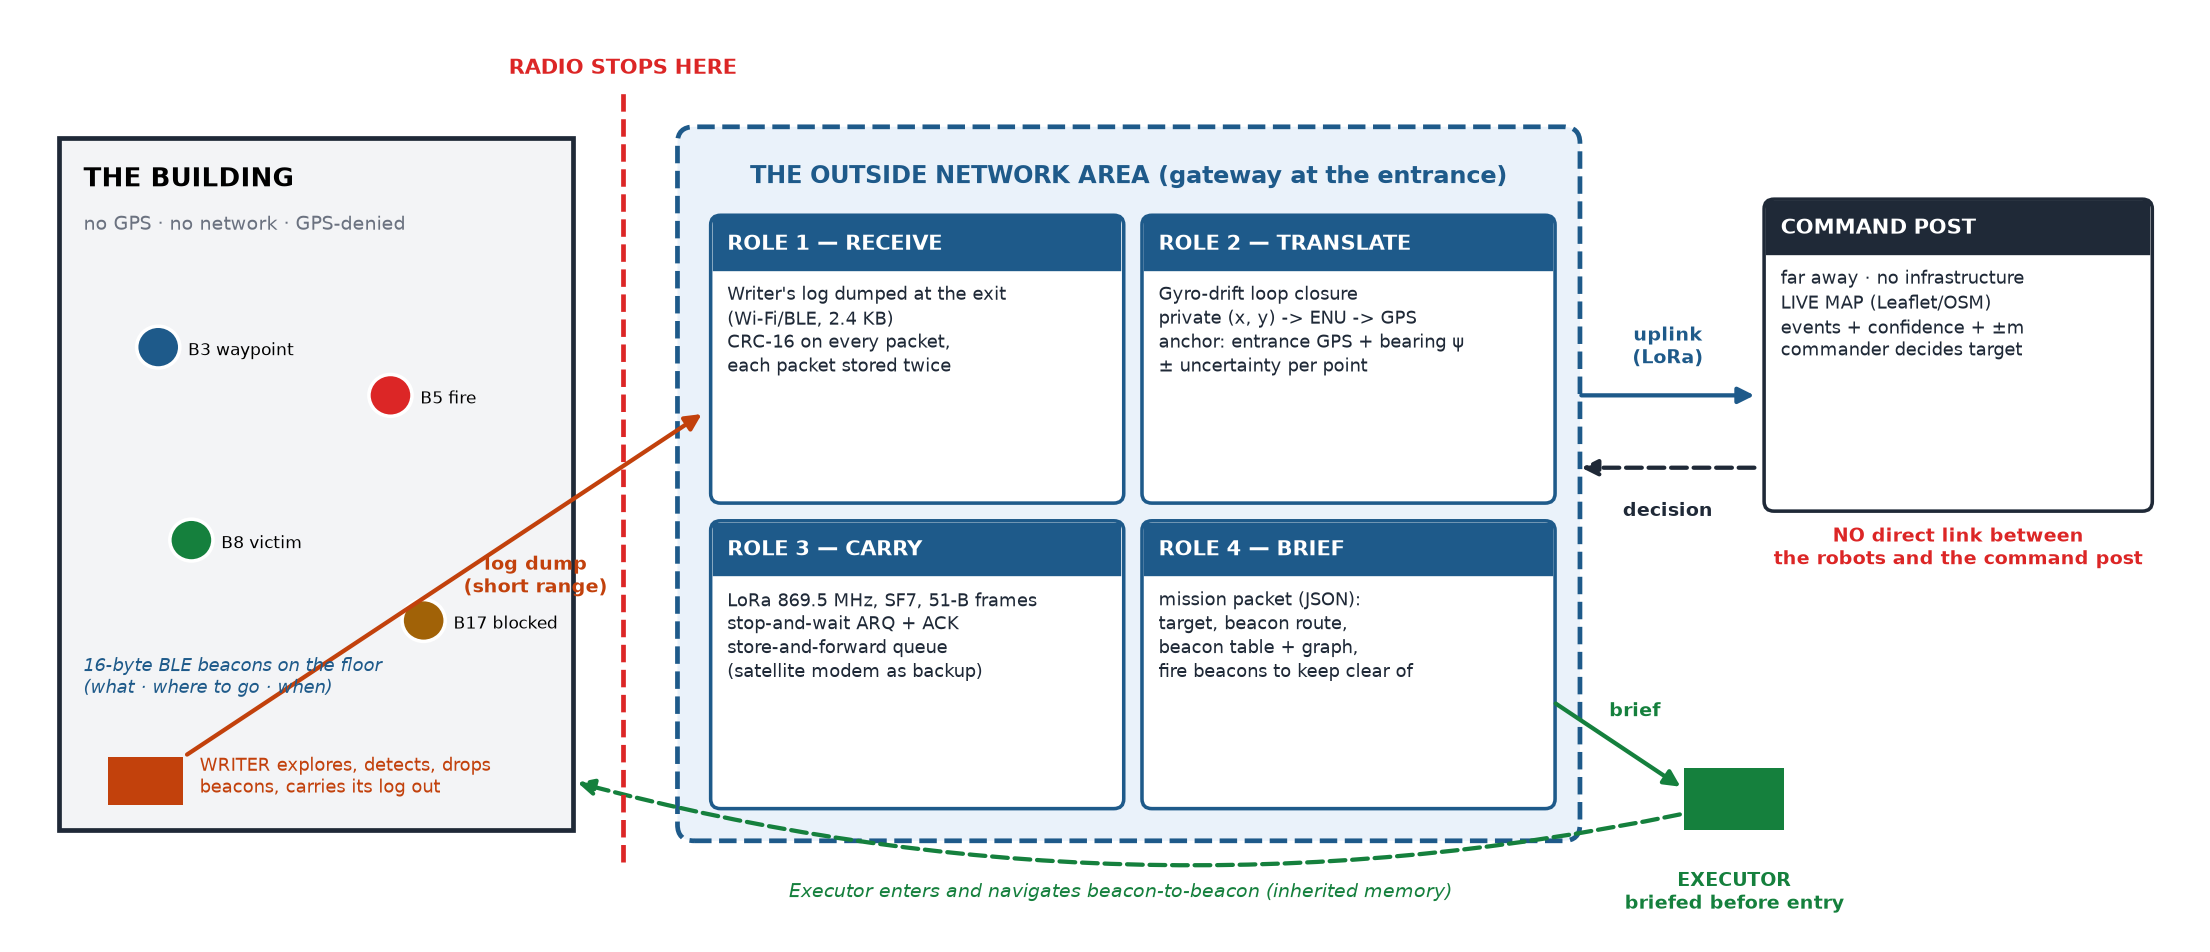
\includegraphics[width=\linewidth]{architecture.png}
\vspace{-14pt}
\caption{Architecture. All inside$\leftrightarrow$outside traffic goes through the ONA; robots never talk to the command post
(this is checked by \texttt{test\_no\_direct\_robot\_to\_command\_post\_link}).}
\label{fig:arch}
\end{figure}
\vspace{-6pt}
\textbf{Mission sequence} (Fig.~\ref{fig:arch}; a sequence diagram is in \texttt{docs/dataflow.png}):
(1)~The Writer drops the exit beacon B0 at the entrance and explores.
(2)~On events, at doorways and every 3\,m, it drops a beacon.
(3)~When its battery or the frontier runs out, it returns and dumps a binary log at the entrance.
(4)~The ONA checks CRCs, estimates odometry drift, converts everything to GPS and builds a beacon graph.
(5)~LoRa frames update the command post's live map; the commander picks a victim; the decision returns to the ONA.
(6)~The ONA briefs the Executor with a route over the beacon graph.
(7)~The Executor navigates using the beacons, confirms the victim and returns.
(8)~Its report goes back through the ONA to the map.

\section{Writer Robot Autonomy}
\begin{minipage}[t]{0.50\linewidth}\vspace{0pt}
The Writer builds an occupancy grid (0.5\,m cells) from a 3\,m, 72-ray lidar. It runs \textbf{frontier
exploration}: it repeatedly drives (A*, 8-connected, no corner cutting) to the nearest known-free cell that borders
unknown space. Decisions:
\begin{itemize}
\item \textbf{Heat no-go zones:} cells localised as burning by the thermal sensor, inflated by one cell, are never entered.
\item \textbf{Battery-aware return:} at each step the robot plans the path home. When
$\text{battery} < 1.3\times\text{cost-to-exit}+15$, it turns back. Coming back is what saves the data and gives the loop closure (§5).
\item \textbf{Beacon budget:} 24 beacons; the last 4 are reserved for events.
\end{itemize}
\end{minipage}\hfill
\begin{minipage}[t]{0.48\linewidth}\vspace{0pt}
\centering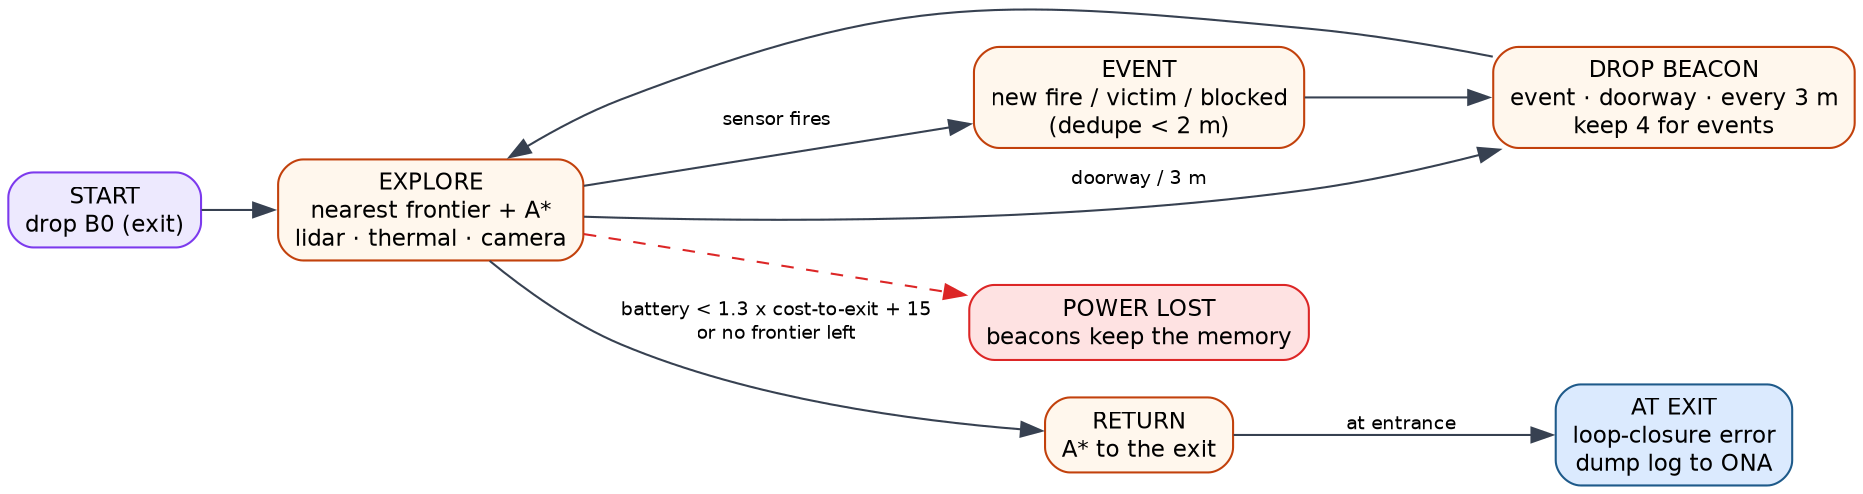
\includegraphics[width=\linewidth]{writer_fsm.png}
\captionof{figure}{Writer decision state machine.}
\end{minipage}

\section{Event Detection and Beacon Deposition}
\begin{tabularx}{\linewidth}{@{}lXl@{}}
\toprule
\textbf{Event} & \textbf{Detection (simulated sensor $\rightarrow$ Phase~2 part)} & \textbf{Severity byte}\\
\midrule
Fire & Air temperature $T=25+\sum 400e^{-d/0.6}$\,°C (line of sight) $>60$\,°C, then hot cells localised in view $\rightarrow$ MLX90614 / AMG8833 & $2(T-25)$\\
Victim & Camera detection $\le2$\,m, line of sight $\rightarrow$ Pi Camera + MobileNet-SSD person detector & $255(1-0.3d/2)$\\
Blocked & Lidar hits debris in a passage $\rightarrow$ lidar / ToF & 255\\
\bottomrule
\end{tabularx}

Events of the same type within 2\,m of a known one are merged. A beacon is also dropped at \textbf{doorways}
(the robot is between two walls), which are the critical navigation points, and every \textbf{3\,m} of travel.
Each new beacon points \texttt{next\_id} to the beacon it can hear that is closest to the exit. The beacons therefore
form a \textbf{tree rooted at the exit}, with extra edges between beacons that hear each other. In the nominal run the
Writer covers 100\,\% of the building in 8.9\,min (106\,m), finds 5/5 events and drops 22 beacons.

\section{Beacon Message and Signal Design}
\begin{figure}[h]
\centering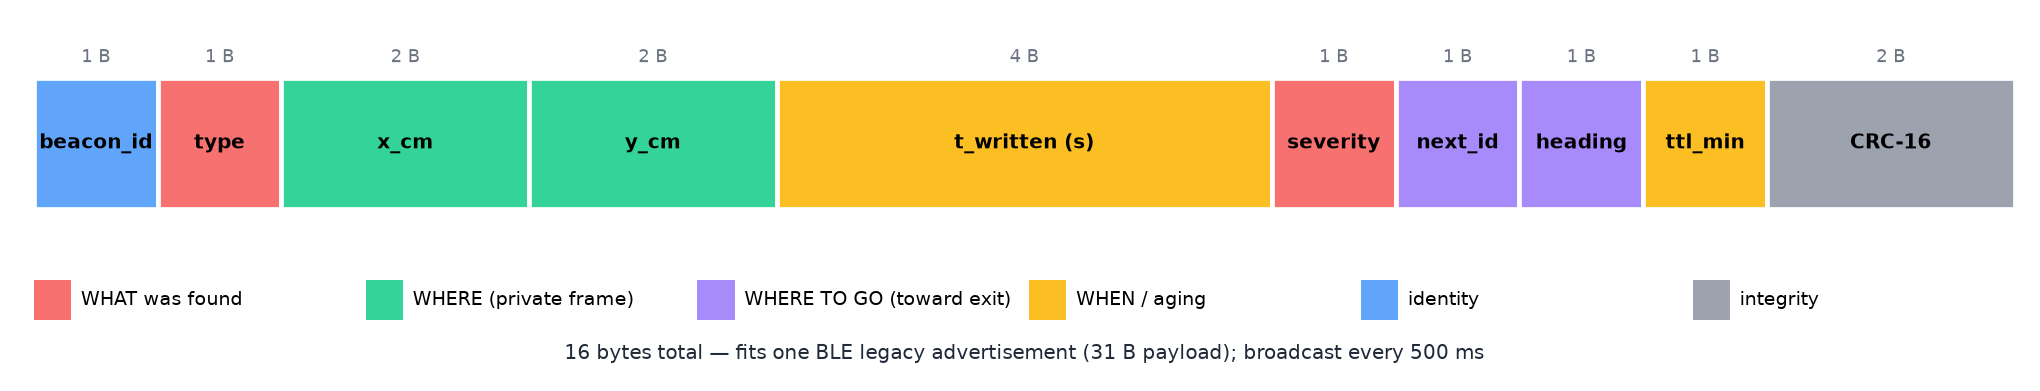
\includegraphics[width=0.92\linewidth]{beacon_packet.png}
\vspace{-6pt}
\caption{16-byte beacon packet (little-endian, CRC-16/CCITT). Position is in the Writer's private frame, in cm.}
\end{figure}
\vspace{-6pt}
\begin{minipage}[t]{0.5\linewidth}\vspace{0pt}
\textbf{Signal.} BLE~5 legacy advertising from an ESP32-C3 on a coin cell. One 16\,B packet every 500\,ms fits the
31\,B advertisement. There is no pairing, so any robot can read it. Range is about 5\,m line of sight; RSSI gives
proximity (arrival $<0.75$\,m). A beacon is \emph{write-once}, so it never needs a receiver or a clock.
\textbf{Message aging} is done by the reader:
$c(t)=\frac{\text{sev}}{255}e^{-\text{age}/\tau}$, and $c=0$ once age $>$ TTL.
Stale beacons are still used for navigation, but their events are shown as \emph{unverified}.
\end{minipage}\hfill
\begin{minipage}[t]{0.46\linewidth}\vspace{0pt}
\centering\tablesize
\begin{tabular}{@{}lccl@{}}
\toprule
Event & $\tau$ & TTL & Why\\\midrule
Fire & 10 min & 30 min & spreads fast\\
Victim & 30 min & 90 min & may move\\
Blocked & 2 h & 4 h & structural\\
Waypoint & $\infty$ & — & geometry\\
\bottomrule
\end{tabular}
\captionof{table}{Per-event aging.}
\end{minipage}

In the simulation the Executor logs, for example, ``\textit{reads B5: fire written 9.8 min ago, confidence 0.14}''.
When the uplink is slow (\texttt{link} scenario), fire confidence falls below the 0.15 threshold and the commander's
risk assessment changes. Aging has a direct effect on decisions.

\section{Frame Translation}
\textbf{Frames.} The private frame has its origin at the entrance, $+x$ into the building and $+y$ to the left. Both
robots start at the same pose, so they share it. The ONA measures the anchor GPS $(\phi_0,\lambda_0)$ and the bearing
$\psi$ of $+x$ (compass or two GPS fixes along the façade):
\[
N = x\cos\psi + y\sin\psi,\quad E = x\sin\psi - y\cos\psi,\quad
\phi = \phi_0 + \frac{N}{R}\cdot\frac{180}{\pi},\quad \lambda = \lambda_0 + \frac{E}{R\cos\phi_0}\cdot\frac{180}{\pi},\quad R=6\,378\,137\text{ m}.
\]
Worked example: $\phi_0{=}36.8000^\circ$, $\lambda_0{=}10.1800^\circ$, $\psi{=}90^\circ$, $(x,y){=}(10,5)$\,m
$\Rightarrow N{=}5$\,m, $E{=}10$\,m $\Rightarrow (36.800045^\circ, 10.180112^\circ)$ (unit-tested).

\begin{figure}[t]
\centering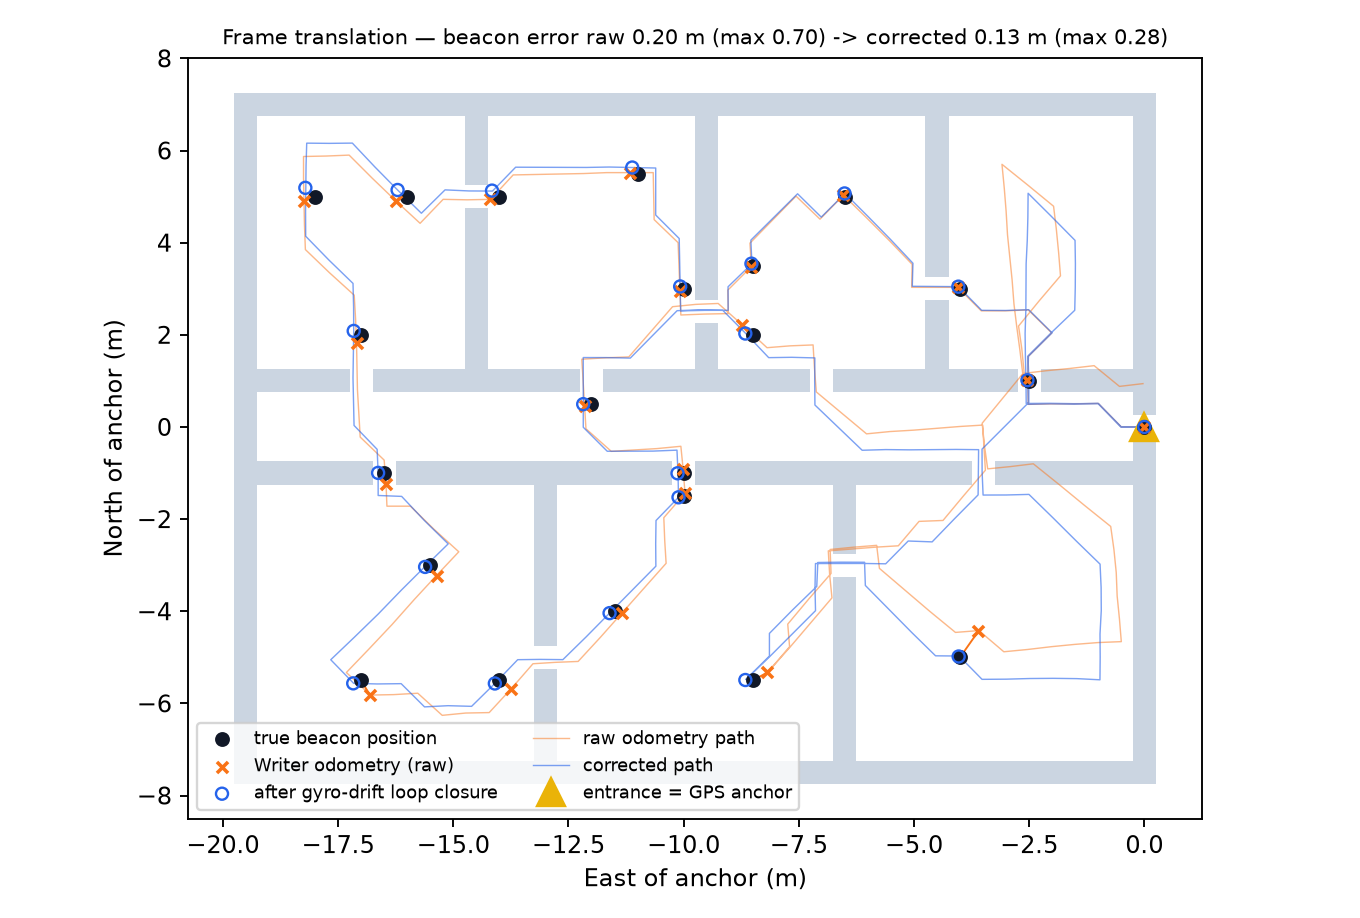
\includegraphics[width=0.62\linewidth]{fig_translation.png}
\vspace{-4pt}
\caption{True vs.\ raw vs.\ corrected beacon positions (ENU around the anchor), nominal run.}
\end{figure}
\textbf{Gyro-drift loop closure (our contribution).} Cheap MEMS gyros drift. We simulate 0.012\,°/s (about 6° per
100\,m) plus a 1.5\,\% wheel scale error and noise. The Writer always ends at the entrance, whose true position is
(0,0). The ONA searches for the drift rate $\beta$ (rad/m) such that re-integrating every odometry step rotated by
$-\beta\cdot\text{odo}$ closes the loop. It then moves every beacon by the correction at the same odometer reading.
The estimate was $\hat\beta=6.08$°/100\,m (true value 6.0).

\medskip
{\centering\tablesize
\begin{tabular}{@{}lcc@{}}
\toprule
Beacon position error & mean & max\\\midrule
Raw odometry (seed 7) & 0.20 m & 0.70 m\\
\textbf{Gyro loop closure} & \textbf{0.13 m} & \textbf{0.28 m}\\
5 seeds, raw $\to$ corrected & 0.25$\to$0.20 & 0.65$\to$0.34\\
Linear spreading (5 seeds) & \multicolumn{2}{c}{worse: 0.25 $\to$ 0.40 mean}\\
\bottomrule
\end{tabular}\par}
\medskip
The classic method of spreading the closure error linearly made things \emph{worse}, because heading drift
\emph{rotates} the path. Modelling the physical cause fixed it. Each GPS point carries a $\pm$ radius, drawn on the
live map.

\section{Outside Network Area}
\begin{tabularx}{\linewidth}{@{}lXX@{}}
\toprule
\textbf{Role} & \textbf{How (simulation, \texttt{sim/ona.py})} & \textbf{Phase~2 hardware}\\\midrule
1 Receive & Binary log dump at the exit (2.4\,KB). Each packet is stored \emph{twice}; the CRC picks the valid copy (4\,\% per-copy corruption injected). & Raspberry Pi~4 Wi-Fi AP; the Writer pushes over TCP when it docks (BLE fallback)\\
2 Translate & Gyro-drift loop closure $\rightarrow$ ENU $\rightarrow$ WGS-84, $\pm$ uncertainty; builds the beacon graph & Pi + u-blox NEO-M8N + compass\\
3 Carry & 51-byte LoRa frames (SF7, 869.5\,MHz, 10\,\% duty-cycle sub-band). 18\,B per beacon record (lat/lon at 1e-7°), 12 path points per frame. Stop-and-wait ARQ with 8 retries, then store-and-forward. & 2$\times$SX1276 (km range line of sight), relay if needed, Iridium SBD fallback\\
4 Brief & Mission JSON: target, route = Dijkstra over the beacon graph (+40\,m penalty near confident fire), beacon table, edges, fire beacons to keep clear of & Same AP, before entry\\
\bottomrule
\end{tabularx}

\textbf{Results:} the nominal map uses \textbf{23 frames (844\,B)}, delivered in 30 transmissions with 7 losses
recovered. At 45\,\% loss it took 64 transmissions and no frame was lost. The \textbf{command post} decodes the frames
into a live Leaflet/OpenStreetMap page (\texttt{out/live\_map.html}) showing events, confidence, age, $\pm$ circles and
both robot paths. The commander scores victims with
$\text{score}=\frac{c_{\text{now}}}{1+\text{route}/30}\times(0.3 \text{ if the route passes within 3\,m of a confident fire})$.
Only the decision goes back down, and it goes to the ONA.

\begin{figure}[h]
\centering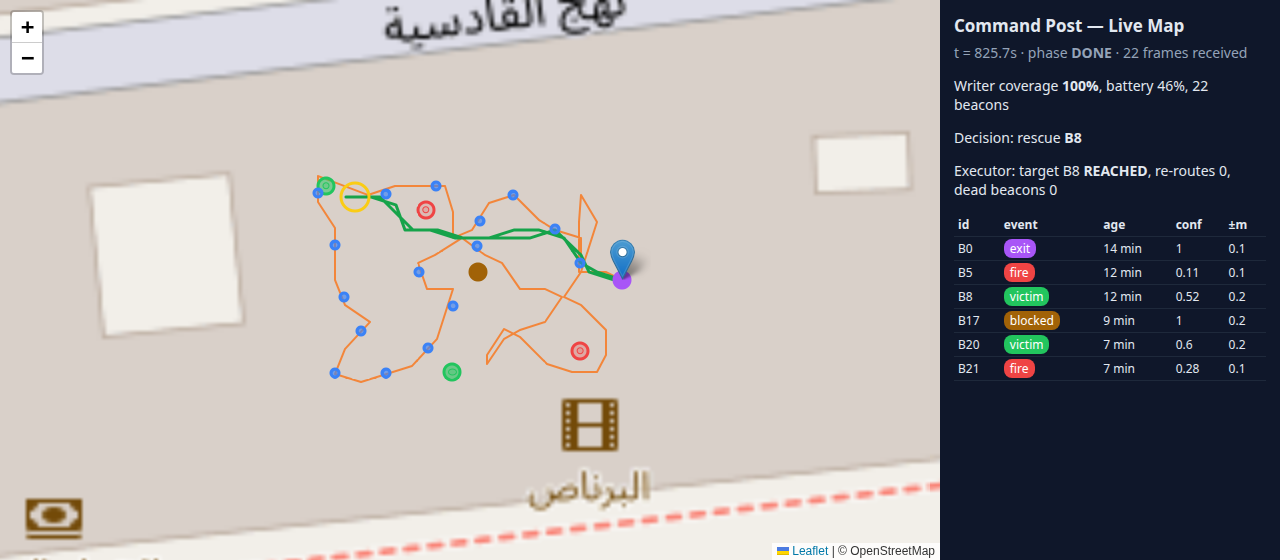
\includegraphics[width=0.82\linewidth]{live_map.png}
\vspace{-4pt}
\caption{Command-post live map (\texttt{out/live\_map.html}, Leaflet/OSM) at the end of the mission. Orange shows the
Writer's corrected path, green the Executor's path, and the yellow ring the reached victim. The side panel lists each
event's age, decayed confidence and $\pm$ error.}
\end{figure}

\section{Executor Robot}
The Executor receives the brief, has \textbf{no map}, and follows the route beacon by beacon. For each beacon it:
plans locally with its own lidar (unknown space treated as free); declares \emph{arrival} when the beacon's RSSI shows
it is $<0.75$\,m away; uses \textbf{RSSI-gradient search} when it reaches the recorded position without being close;
and re-localises when it drives over a beacon. If a beacon is \textbf{silent} at its recorded position for 8 steps, it
is declared dead and the robot \textbf{re-routes} over the graph from a virtual node at its current position. If the
local path to the next beacon is $>3\times$ longer than expected, that \textbf{edge is marked blocked} and removed. At
the target it walks to the reported event position, \textbf{confirms the victim with its camera} ($\le1$\,m), drops the
aid kit and returns. In \textbf{recovery mode} (Writer lost) it explores, reads the Writer's beacons, goes to the first
victim beacon it hears, and brings all beacons read back to the ONA.

\section{Simulation Demo and Results}
\begin{minipage}[t]{0.56\linewidth}\vspace{0pt}
\centering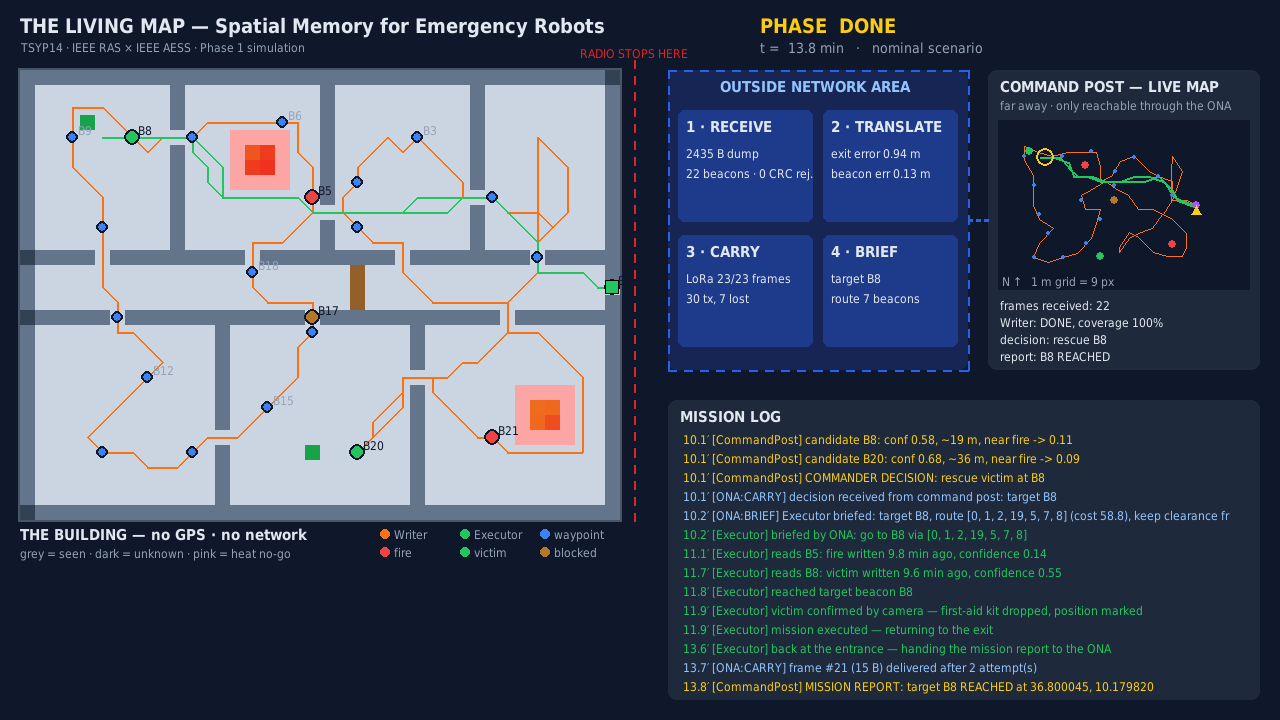
\includegraphics[width=\linewidth]{demo_final.png}
\captionof{figure}{Simulator (Pygame) at the end of the nominal mission: building with the Writer's (orange) and
Executor's (green) trails, beacons, the ONA's 4 roles, the command-post live map and the mission log.}
\end{minipage}\hfill
\begin{minipage}[t]{0.42\linewidth}\vspace{0pt}
\centering\tablesize
\begin{tabular}{@{}ll@{}}
\toprule
Metric (seed 7) & Value\\\midrule
Writer coverage / time & 100\,\% / 8.9 min\\
Distance / beacons & 106 m / 22\\
Events found & 5/5 (2F, 2V, 1 blocked)\\
Exit (closure) error & 0.94 m\\
Beacon error (corr.) & 0.13 m mean\\
Uplink & 23 frames, 844 B, 30 tx\\
Decision & victim B8 (0.58 conf., 19 m)\\
Executor & 41 m, 3.4 min, confirmed\\
Whole mission & 13.8 min\\
Tests & 21/21 pass\\
\bottomrule
\end{tabular}
\captionof{table}{Nominal mission results.}
\end{minipage}

\smallskip
Run with \texttt{python -m sim.main} (options \texttt{--fail beacon|block|writer|link|battery}, \texttt{--headless}, \texttt{--record}).
The 40$\times$30 building (20$\times$15\,m) has two fires, two victims and debris that cuts the main corridor, so every
route has to pass through rooms. The simulator uses the \emph{same} packet codec, translation, framing and routing code
that will run on the ONA Pi and the robots in Phase~2.

\section{Failure Cases}
{\tablesize
\begin{tabularx}{\linewidth}{@{}lXXl@{}}
\toprule
\textbf{Failure} & \textbf{Detection} & \textbf{Response} & \textbf{Simulated}\\\midrule
Writer dies inside & No return within 15 min & Executor in recovery mode reads the Writer's beacons & \checkmark\ success (61\,\% explored)\\
Beacon battery dies & Silent at its position for 8 steps & Mark dead, re-route on the graph & \checkmark\ B19 dead $\rightarrow$ [18,7,8]\\
Doorway collapses later & Lidar debris, path $>3\times$ expected & Local detour / remove edge & \checkmark\ success\\
LoRa link degraded (45\,\%) & Missing ACKs & ARQ, 8 retries, store-and-forward & \checkmark\ 64 tx, 0 lost\\
Low battery & $1.3\times$ cost-to-exit rule & Early return, partial map still briefs & \checkmark\ 43\,\% coverage, success\\
Corrupted packet & CRC-16 & Duplicate copy used & \checkmark\ always on\\
Odometry drift & Loop-closure error & Gyro drift removed, $\pm$ circles & \checkmark\ max 0.70$\to$0.28 m\\
Stale information & age $>$ TTL / low $c$ & Unverified, lower priority & \checkmark\ always on\\
Wrong anchor $\psi$ & Points outside footprint & Re-measure from 2 GPS fixes & design\\
No decision received & Downlink timeout & ONA default policy & design\\
\bottomrule
\end{tabularx}}

\section{Implementation Plan (Phase 2) and Innovation}
\begin{minipage}[t]{0.55\linewidth}\vspace{0pt}
{\tablesize
\begin{tabular}{@{}ll@{}}
\toprule
Weeks (2026) & Milestone\\\midrule
6–19 Oct & Hardware, both chassis, PID, ESP32-C3 beacons\\
20–26 Oct & Writer odometry + mapping; ONA dump + translation\\
27 Oct–2 Nov & Frontier exploration, sensors, drop magazine\\
3–9 Nov & LoRa ONA$\leftrightarrow$command post, live map, range test\\
10–16 Nov & Executor beacon navigation + re-routing\\
17–23 Nov & Integration in a mock building\\
24–30 Nov & Failure tests, user manual, pitch\\
\bottomrule
\end{tabular}}

\smallskip
Bill of materials: about 1,300–1,600\,TND (2 chassis, 2 Pi~4, ESP32-S3, ToF/lidar, IMUs, thermal, camera,
12 beacons, 2 LoRa, GPS). Details in \texttt{docs/implementation\_plan.md}.
\end{minipage}\hfill
\begin{minipage}[t]{0.42\linewidth}\vspace{0pt}
\textbf{Innovation}
\begin{itemize}
\item Knowledge \textbf{outlives the robot}: battery-aware return plus write-once beacons, shown working when the Writer dies.
\item Beacons form a \textbf{navigation graph} (\texttt{next\_id} tree + neighbour edges), not isolated markers.
\item \textbf{Gyro-drift loop closure}, which halves the maximum error; the naïve method fails.
\item \textbf{Per-event aging} that changes the commander's decisions.
\item Double-copy dump, CRC and LoRa store-and-forward, so \textbf{nothing is silently lost}.
\end{itemize}
\end{minipage}

\end{document}
